\subsection{Output signals for different input signals}

To prove that the transmitter works correctly and to obtain performance results the output for different input signals was observed. Figure \ref{fig:alternating_data} shows the transient waveform for alternating data at the TX output for \unit[6]{UI}. The eye diagram over \unit[5000]{UI} for a PRBS15 data pattern is given by figure \ref{fig:eye_prbs15}. The eye is not shown for \unit[10000]{UI} as we ran out of disk space and therefore could not run the simulation longer (we have to use cadence on the SOC machine where we only have a quota of \unit[4]{GB}).\\
In figure \ref{fig:wc_eye} the eye for the worst case data pattern of the transmitter is drawn. All bits transmitted in the simulation are shown in the eye diagram. As we used a long wc pattern this results in many traces. Only the two which close the eye the most are the actual worst-case one and zero bits of all bits transmitted for the worst-case pattern.

\begin{figure}[H]
  \centering
  \subfigure[with {\unit[6]{dB}} equalization]
  {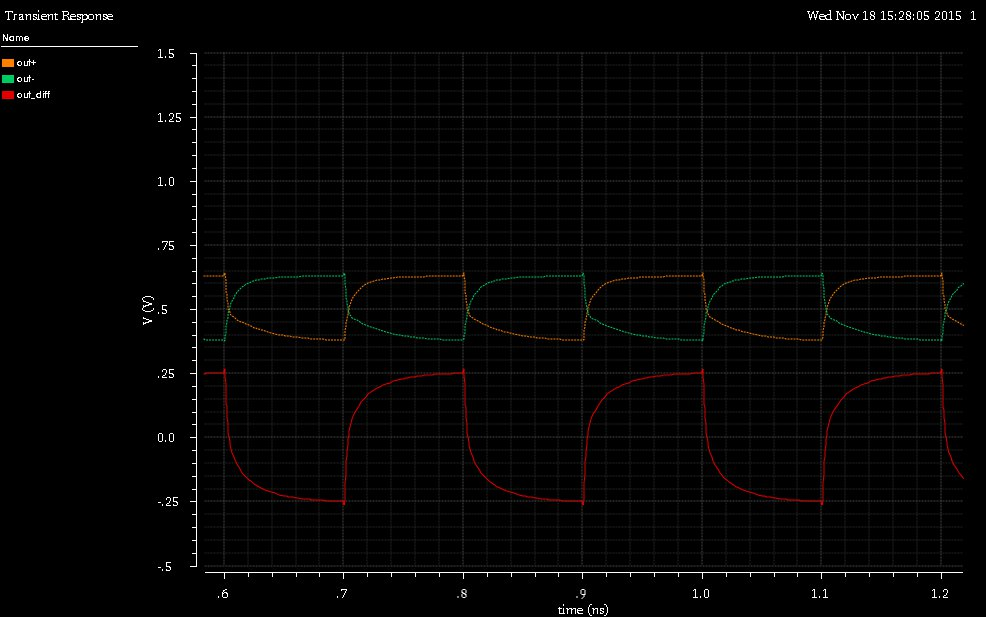
\includegraphics[scale=0.3]{img/alternating_data.jpg}}
  \subfigure[equalization turned off]
  {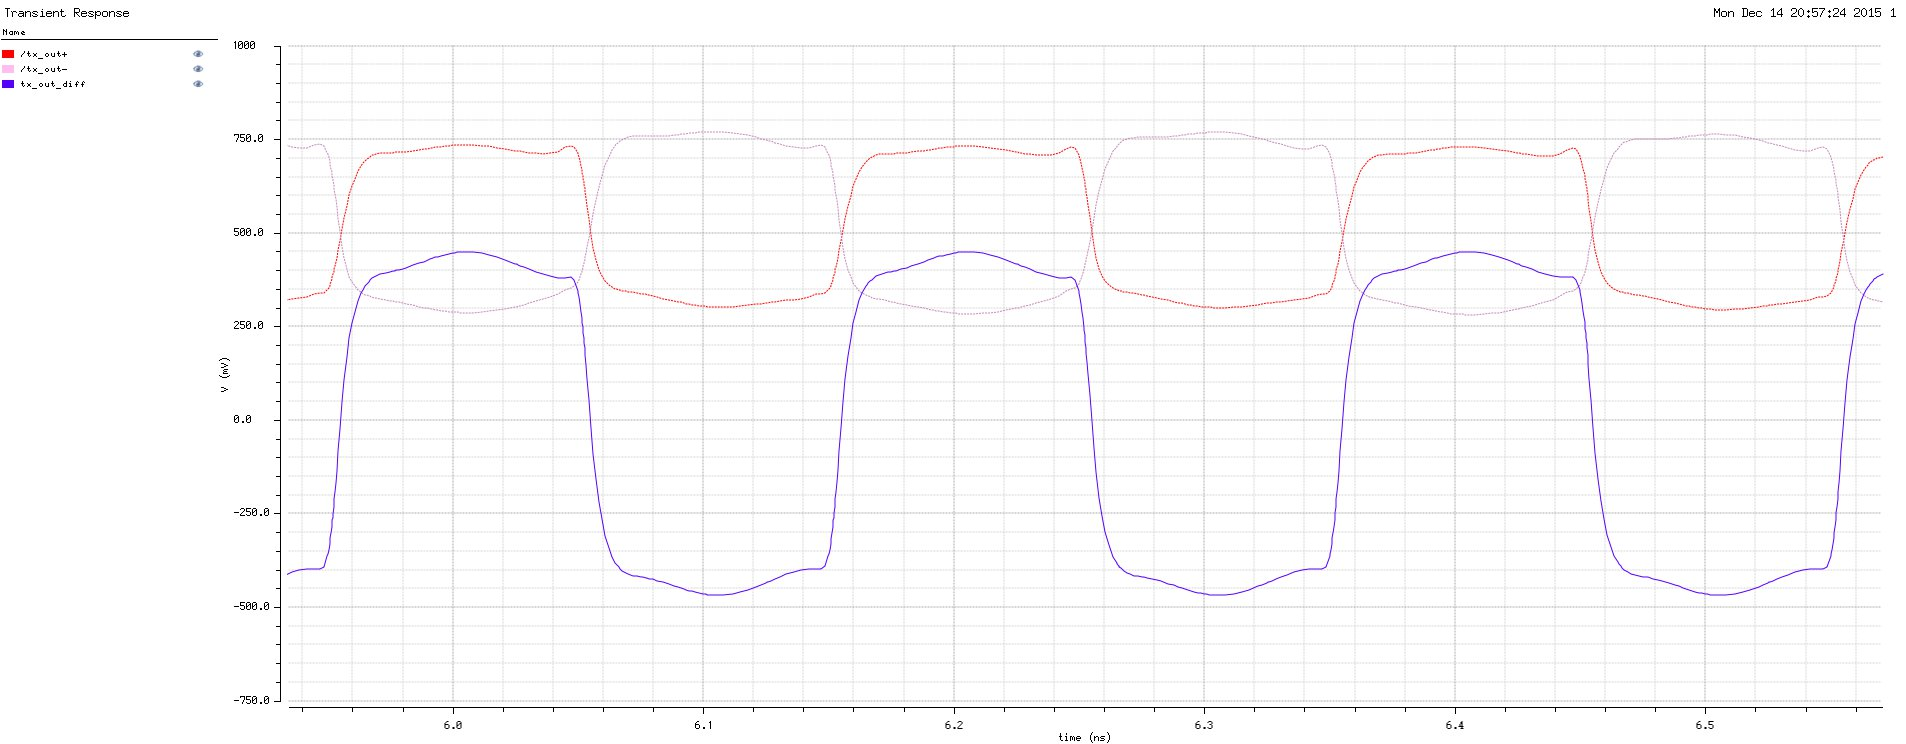
\includegraphics[scale=0.3]{img/alternating_data_no_eq.jpg}}
  \caption{Transmitter output for alternating data at the input}
  \label{fig:alternating_data}
\end{figure}

\begin{figure}[H]
  \centering
  \subfigure[10Gb/s at 1V]
  {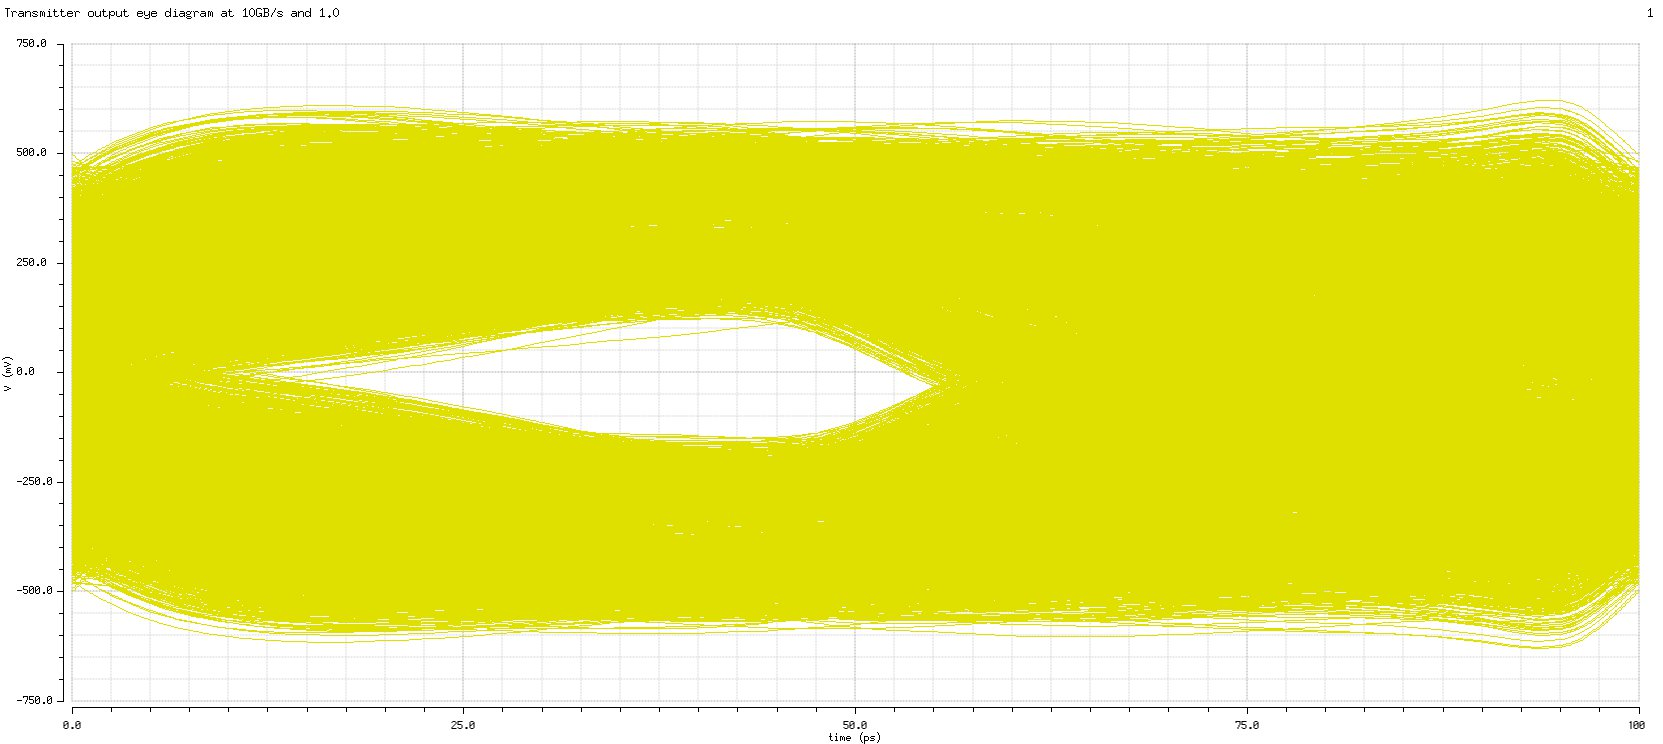
\includegraphics[scale=0.4]{img/eye_tx_10gbs_5000.jpg}}
  \subfigure[2Gb/s at 0.7V]
  {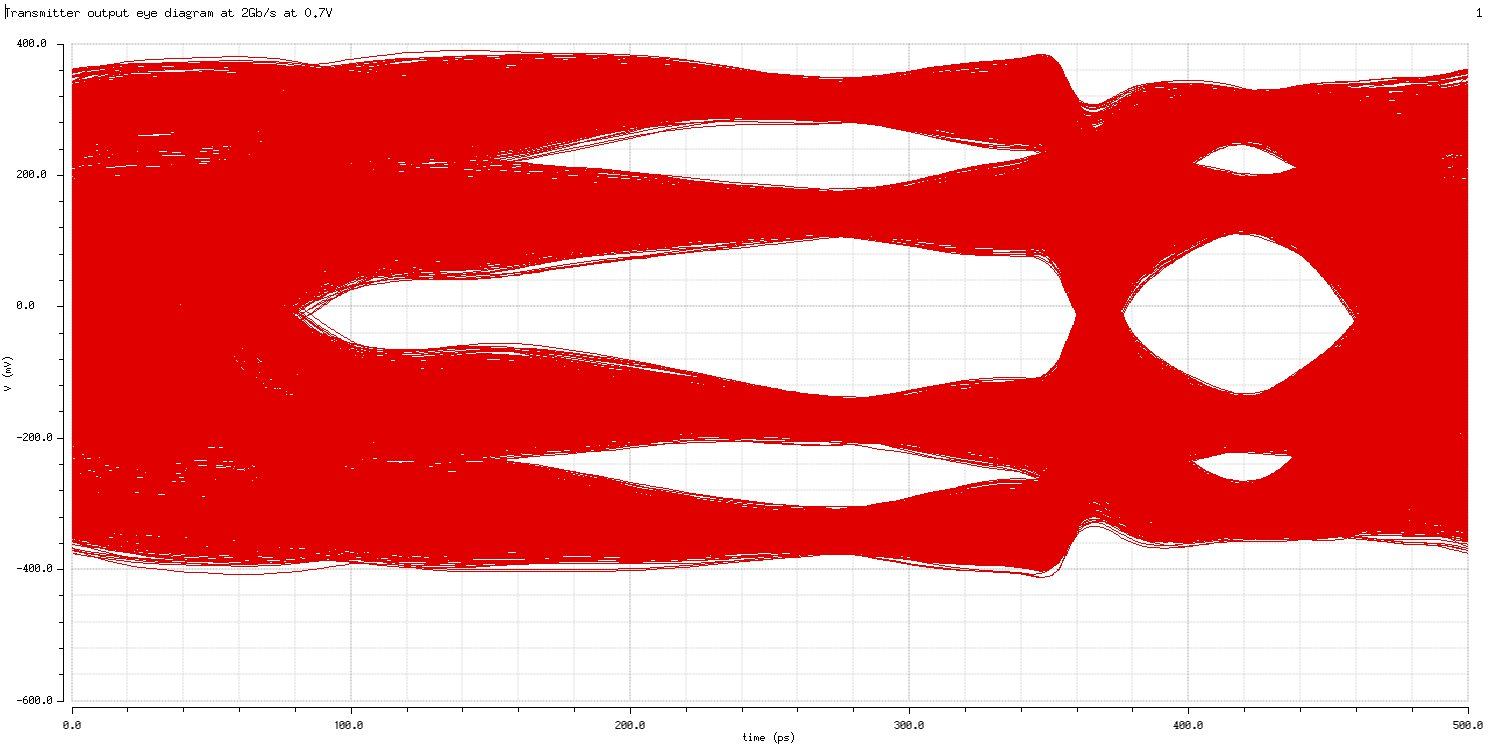
\includegraphics[scale=0.4]{img/eye_tx_2gbs_5000.jpg}}
  \caption{Eye diagram over \unit[5000]{bits} for PRBS15 data pattern}
  \label{fig:eye_prbs15}
\end{figure}

\begin{figure}[H]
  \centering
  {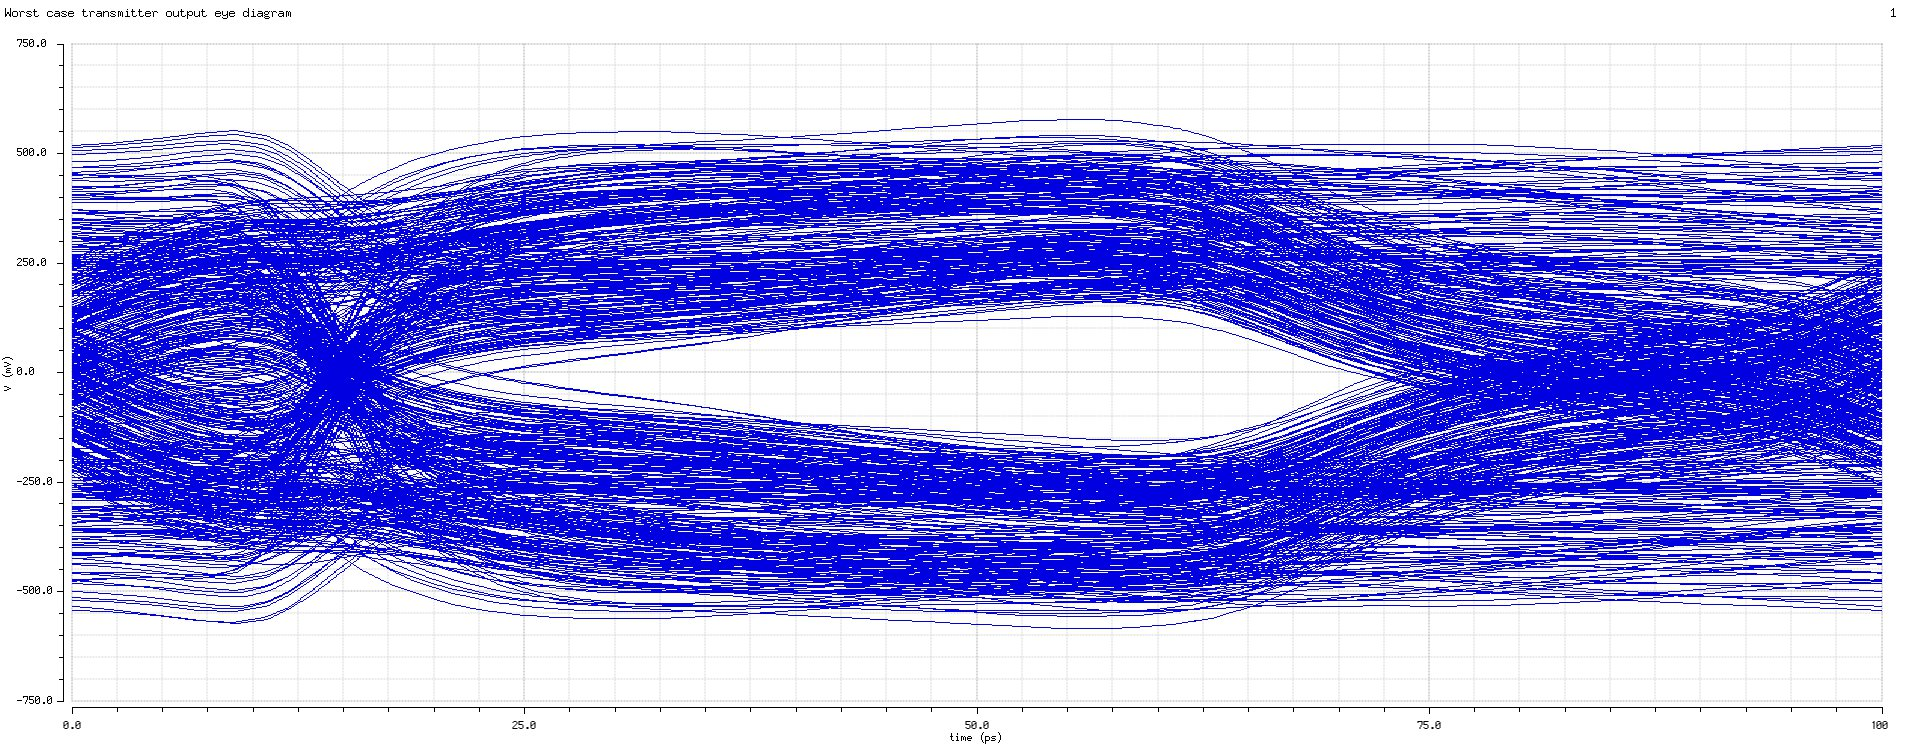
\includegraphics[scale=0.35]{img/wc_eye_tx.jpg}}
  \caption{Worst case eye diagram at the transmitter output}
  \label{fig:wc_eye}
\end{figure}